\documentclass[]{book}
\usepackage{lmodern}
\usepackage{amssymb,amsmath}
\usepackage{ifxetex,ifluatex}
\usepackage{fixltx2e} % provides \textsubscript
\ifnum 0\ifxetex 1\fi\ifluatex 1\fi=0 % if pdftex
  \usepackage[T1]{fontenc}
  \usepackage[utf8]{inputenc}
\else % if luatex or xelatex
  \ifxetex
    \usepackage{mathspec}
  \else
    \usepackage{fontspec}
  \fi
  \defaultfontfeatures{Ligatures=TeX,Scale=MatchLowercase}
\fi
% use upquote if available, for straight quotes in verbatim environments
\IfFileExists{upquote.sty}{\usepackage{upquote}}{}
% use microtype if available
\IfFileExists{microtype.sty}{%
\usepackage{microtype}
\UseMicrotypeSet[protrusion]{basicmath} % disable protrusion for tt fonts
}{}
\usepackage[margin=1in]{geometry}
\usepackage{hyperref}
\hypersetup{unicode=true,
            pdftitle={Systems Pathology: Muscle System},
            pdfauthor={Russell Fraser},
            pdfborder={0 0 0},
            breaklinks=true}
\urlstyle{same}  % don't use monospace font for urls
\usepackage{natbib}
\bibliographystyle{apalike}
\usepackage{longtable,booktabs}
\usepackage{graphicx,grffile}
\makeatletter
\def\maxwidth{\ifdim\Gin@nat@width>\linewidth\linewidth\else\Gin@nat@width\fi}
\def\maxheight{\ifdim\Gin@nat@height>\textheight\textheight\else\Gin@nat@height\fi}
\makeatother
% Scale images if necessary, so that they will not overflow the page
% margins by default, and it is still possible to overwrite the defaults
% using explicit options in \includegraphics[width, height, ...]{}
\setkeys{Gin}{width=\maxwidth,height=\maxheight,keepaspectratio}
\IfFileExists{parskip.sty}{%
\usepackage{parskip}
}{% else
\setlength{\parindent}{0pt}
\setlength{\parskip}{6pt plus 2pt minus 1pt}
}
\setlength{\emergencystretch}{3em}  % prevent overfull lines
\providecommand{\tightlist}{%
  \setlength{\itemsep}{0pt}\setlength{\parskip}{0pt}}
\setcounter{secnumdepth}{5}
% Redefines (sub)paragraphs to behave more like sections
\ifx\paragraph\undefined\else
\let\oldparagraph\paragraph
\renewcommand{\paragraph}[1]{\oldparagraph{#1}\mbox{}}
\fi
\ifx\subparagraph\undefined\else
\let\oldsubparagraph\subparagraph
\renewcommand{\subparagraph}[1]{\oldsubparagraph{#1}\mbox{}}
\fi

%%% Use protect on footnotes to avoid problems with footnotes in titles
\let\rmarkdownfootnote\footnote%
\def\footnote{\protect\rmarkdownfootnote}

%%% Change title format to be more compact
\usepackage{titling}

% Create subtitle command for use in maketitle
\newcommand{\subtitle}[1]{
  \posttitle{
    \begin{center}\large#1\end{center}
    }
}

\setlength{\droptitle}{-2em}

  \title{Systems Pathology: Muscle System}
    \pretitle{\vspace{\droptitle}\centering\huge}
  \posttitle{\par}
    \author{Russell Fraser}
    \preauthor{\centering\large\emph}
  \postauthor{\par}
      \predate{\centering\large\emph}
  \postdate{\par}
    \date{2019-02-20}

\usepackage{booktabs}

\begin{document}
\maketitle

{
\setcounter{tocdepth}{1}
\tableofcontents
}
\chapter*{About}\label{about}
\addcontentsline{toc}{chapter}{About}

These represent the course notes for the skeletal muscle system for VETM
2220. They are broken down into several sections based on disease
process.

\subsection*{Contact me}\label{contact-me}
\addcontentsline{toc}{subsection}{Contact me}

Please don't hesitate to get in touch if you have any questions.

\begin{itemize}
\tightlist
\item
  Phone: 902-620-5183
\item
  E-mail: \href{mailto:rufraser@upei.ca}{\nolinkurl{rufraser@upei.ca}}
\item
  Office: 414N
\end{itemize}

\begin{description}
\tightlist
\item[Abc]
Definition 1 sadf
\end{description}

\chapter{Introduction}\label{intro}

\section{The anatomy of muscle}\label{the-anatomy-of-muscle}

The basic structural unit of muscle is the \textbf{myofiber}, which
represents a single, long, tubular cell (Figure
\ref{fig:muscle-structure}). Within each myofiber are many tightly
packed \textbf{myofibrils}, which are composed of actin and myosin
filaments, and which form the contractile machinery of the muscle. The
cytoplasm of a myofiber is known as the \textbf{sarcoplasm}, while the
cell membrane is called the \textbf{sarcolemma}. Each myofiber is
surrounded by a small amount of connective tissue called the
\textbf{endomysium}. Multiple myofibers form a \textbf{fasicle} that is
surrounded by another layer of connective tissue, the
\textbf{perimysium}. Finally, multiple fasicles form a muscle. It is the
arrangment of myofibrils that form the striated appearance of skeletal
muscle that can be appreciated under light microscopy (Figure
\ref{fig:muscle-histo}).

\begin{figure}

{\centering 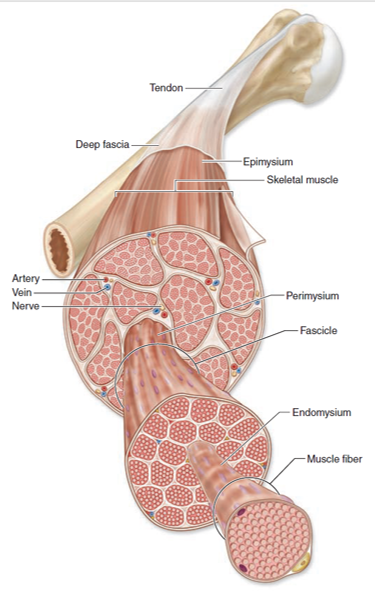
\includegraphics[width=0.6\linewidth]{images/muscle_structure} 

}

\caption{Structure and anatomy of muscle}\label{fig:muscle-structure}
\end{figure}

\begin{figure}

{\centering 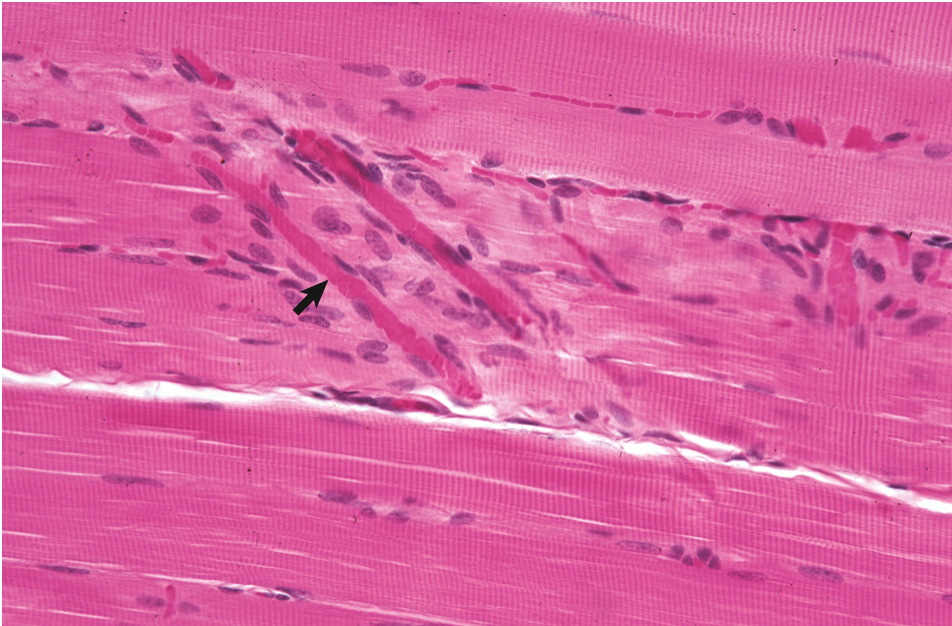
\includegraphics[width=0.8\linewidth]{images/muscle_histo} 

}

\caption{Normal skeletal muscle demonstrating striations. The arrow indicates a small capillary.}\label{fig:muscle-histo}
\end{figure}

Skeletal muscle is characteristically multinucleated: each myofiber can
have 100s of nuclei scattered along its length, almost always found
along the periphery of the cell. Each nucleus within a myofiber controls
a specific portion of the myofiber, and each nucleus acts independently.
Nuclei within muscle fibers are \emph{terminally differentiated},
meaning they can no longer divide, thus limiting the capacity for
regeneration. On the other hand, having multiple nuclei within a cell
provides a distinct benefit: localized damage, affecting a small number
of nuclei, will not necessarilly kill the entire cell, giving the
myofiber an opportunity to regenerate.

\section{The function of muscle}\label{the-function-of-muscle}

The contraction of muscle is a complex, orchestrated process in which
myofilaments (the components of myofibrils) undergo a conformational
change that results. The contraction of muscle is initiated at the
\textbf{motor end plate} by the release of acetylcholine into the
neuromuscular junction. This depolarizes the myofiber, resulting in the
release of \textbf{calcium} from teh sarcoplasmic reticulum. It is the
binding of calcium to the myofilament tropononin that results in the
contraction of the sarcomere. Importantly, calcium must be pumped back
into the sarcoplasmic reticulum in an ATP-dependent process. Once this
occurs, the muscle enters into a relaxed, resting state.

\section{Reactions of muscle}\label{reactions-of-muscle}

\subsection{Atrophy}\label{atrophy}

\subsubsection{Neurogenic}\label{neurogenic}

\subsubsection{Disuse}\label{disuse}

\subsubsection{Nutritional}\label{nutritional}

\subsection{Hypertrophy}\label{hypertrophy}

\subsection{Necrosis and regeneration}\label{necrosis-and-regeneration}

\section{Gross evaluation of muscle}\label{gross-evaluation-of-muscle}

Although important, the gross examination of muscles during a necropsy
can be underwhelming, and if muscular disease is suspected, samples of
muscle should \emph{always} be submitted for histopathology. During a
gross examination of a carcass, muscles should be evaluated for changes
in size, texture, and colour. Muscles can be bigger (hypertrophied) or,
more commonly, smaller (atrophied), or normal. Difficulty in assessing
the normal size of muscles for different species and breeds can be aided
by comparing with normal animals, or, if unilateral disease is present,
with the contralateral side.

Changes in the colour of muscle are common, are frequently artifactual,
and are dependent on blood perfusion, age, and species. Commonly
observed colour changes, along with potential causes, are listed below.

\begin{itemize}
\tightlist
\item
  Pale muscles:

  \begin{itemize}
  \tightlist
  \item
    Normal in young animals
  \item
    Common in anemic animals
  \item
    Can be due to necrosis (ischemic)
  \item
    Denervation
  \item
    If streaking observed, usually due to necrosis and mineralization.
  \end{itemize}
\item
  Dark red:

  \begin{itemize}
  \tightlist
  \item
    Congestion or hemorrhage
  \item
    Hemorrhagic necrosis
  \item
    Inflammation
  \item
    Hypostatic congestion (i.e.~blood pooling due to gravity, and
    artifact found in postmortem examinations)
  \end{itemize}
\item
  Green:

  \begin{itemize}
  \tightlist
  \item
    Putrefaction (rot)
  \item
    Eosinophilic inflammation
  \end{itemize}
\end{itemize}

The texture of diseased muscle can range from soft to hard
(mineralized). Soft muscle can be indicative of necrosis, or potentially
fat infiltration.

\section{Biopsy techniques}\label{biopsy-techniques}

As noted above, a biopsy of muscle should always accompany any suspected
muscular disease. Muscle is highly susceptible to artifact, but proper
preparation of the sample can help in ensuring a diagnostic sample.
Muscle retains the ability to contract after biopsy/death, and this
contraction can result in artifactual histological changes that mimic
true pathological changes. These changes, noted as \emph{contraction
band artifact}, can be prevented relatively easily: shortly after
removal, secure the muscle to a rigid surface prior to fixation. A
simple and manageable technique whether in the field or clinic is to
place a strip of muscle along a tongue depressor, and anchor it into
place using two needles (FIGURE XXX GET PICTURE), prior to placing the
sample in formalin. As a general rule, a muscle biopsy should not exceed
\textasciitilde{} 1 cm in diameter (with myofibers running lengthwise).

\chapter{Literature}\label{literature}

Here is a review of existing methods.

\chapter{Methods}\label{methods}

We describe our methods in this chapter.

\chapter{Applications}\label{applications}

Some \emph{significant} applications are demonstrated in this chapter.

\section{Example one}\label{example-one}

\section{Example two}\label{example-two}

\chapter{Final Words}\label{final-words}

We have finished a nice book.

\bibliography{book.bib,packages.bib}


\end{document}
